\documentclass[submit]{harvardml}

% FDV: Update dates 
\course{CS181-S20}
\assignment{Assignment \#3}
\duedate{11:59pm March 6, 2020}

\usepackage[OT1]{fontenc}
\usepackage[colorlinks,citecolor=blue,urlcolor=blue]{hyperref}
\usepackage[pdftex]{graphicx}
\usepackage{subfig}
\usepackage{fullpage}
\usepackage{amsmath}
\usepackage{amssymb}
\usepackage{color}
\usepackage{soul}
\usepackage{todonotes}
\usepackage{listings}
\usepackage{common}
\usepackage{enumitem}
\usepackage{bm}
\newcommand{\B}{\text{B}}
\newcommand{\Beta}{\text{Beta}}

\usepackage[mmddyyyy,hhmmss]{datetime}

\definecolor{verbgray}{gray}{0.9}

\lstnewenvironment{csv}{%
  \lstset{backgroundcolor=\color{verbgray},
  frame=single,
  framerule=0pt,
  basicstyle=\ttfamily,
  columns=fullflexible}}{}

\begin{document}

\begin{center}
{\Large Homework 3: Bayesian Methods, Neural Networks, and Practical Supervised Learning}\\
\end{center}

\subsection*{Introduction}

This homework is about Bayesian methods, Neural Networks, and practical supervised
learning.  Section 2.9 in the textbook as well as reviewing MLE and MAP will be useful for Q1. Chapter 4 in the textbook will be useful for Q2.

Please type your solutions after the corresponding problems using this
\LaTeX\ template, and start each problem on a new page.

Please submit the \textbf{writeup PDF to the Gradescope assignment `HW3'}. Remember to assign pages for each question. 

Please submit your \textbf{\LaTeX file and code files to the Gradescope assignment `HW3 - Supplemental'}. 

You can use a \textbf{maximum of 2 late days} on this assignment.  Late days will be counted based on the latest of the two submissions.
\\

\newpage

\begin{problem}[Bayesian Methods]

  This question helps to build your understanding of making
  predictions with a maximum-likelihood estimation (MLE), a maximum a
  posterior estimator (MAP), and a full posterior predictive.

  Consider a one-dimensional random variable $x \sim \mu + \epsilon$,
  where it is known that $\epsilon \sim N(0,\sigma^2)$.  Suppose we
  have a prior $\mu \sim N(0,\tau^2)$ on the mean.  Use $\sigma^2 = 1$
  and $\tau^2 = 5$.  

  In this problem, we see 14 independent samples of $x$ to yield data
  $$D = 3.3, 3.5, 3.1, 1.8, 3.0, 0.74, 2.5, 2.4, 1.6, 2.1, 2.4, 1.3, 1.7, 0.19$$
    
  \textit{Make sure to include all required plots in your PDF.}

\begin{enumerate}

\item We are interested in the predictive distribution of a new datapoint $x^*$ given our observed data $D$, $p(x^*|D)$.
  Write down the expression for the full posterior predictive distribution: $$p(x|D) = \int p(x|\mu)p(\mu|D) d\mu$$
  
  There are two ways to do this problem. One involves actually doing out this integral, which has been well studied and there are resources that can guide you through it (http://www.tina-vision.net/docs/memos/2003-003.pdf). The second involves using the representation of $x$ and calculating the posterior of $\mu$.
  
 \item The full posterior predictive distribution is often difficult to calculate because we need to marginalize out the parameters (here, the parameter is $\mu$). We can mitigate this problem by plugging in a point estimate of $\mu$. Find the estimates of $p(x|D) \approx p(x|\mu^*)$ for $\mu^* = \mu_{MLE}$ and $\mu^* = \mu_{MAP}$.
   
\item Plot how the above 3 distributions change after each data point is
  gathered.  You will have a total of 15 plots (they can be small,
  e.g. in a 3x5 grid).  The x-axis of each plot will be the $x$ value
  and the y-axis the density.  You can make one plot for each
  estimator, or combine all three estimators onto one plot with a
  different colored line for each estimator.
  
    
\item How do the means of the predictive distributions vary with more
  data?  How do the variances vary?  Interpret the differences you see
  between the three different estimators.
  
  \item Does the ordering of the data matter for the final predictive
  distributions?  

  \item Compute the marginal likelihood of the training data $p(D)$.
  Hint: Note that the required integral looks like an unnormalized
  Gaussian distribution, and take advantage of the fact that
  integrating over a normalized Gaussian distribution is equal to 1.

  \item Now consider an alternate model in which we were much more sure
  about the mean: $\mu \sim N(0,\tau^2)$, where $\tau^2 = 0.1$.
  Compute the marginal likelihood $p(D)$ for this model.  Which of the
  two models has a higher marginal likelihood? Interpret this result.
\end{enumerate}

\end{problem}
\newpage
\subsection*{Solution}
 \begin{enumerate}
     \item 
     \begin{equation*}
         p(x^*|D) = \int \mcN(x^*|\mu, \sigma^2) \mcN(\mu | \mu_{n}, \sigma_{n}^2)
     \end{equation*}
     \begin{equation*}
         = \mcN(x^* | \mu_{n}, \sigma_{n}^2 + \sigma^2)
     \end{equation*}
     \begin{equation*}
         \sigma_{n}^2 = \frac{\sigma^2\tau^2}{n\tau^2 + \sigma^2} \hspace{2cm} \mu_{n} = \frac{n\tau^2\Bar{x}}{n\tau^2 + \sigma^2}
     \end{equation*}
     \begin{equation*}
         p(x^*|D) = \mcN(x^* | \frac{n\tau^2\Bar{x}}{n\tau^2 + \sigma^2}, \frac{\sigma^2\tau^2}{n\tau^2 + \sigma^2} + \sigma^2) = \mcN(x^* | 2.0866, 1.0704)
     \end{equation*}
     \item
     \begin{equation*}
     \mu_{MAP} = \arg\max_{\mu} p(\mu|D)
     \end{equation*}
     \begin{equation*}
     = \arg\max_{\mu} p(D|\mu) p(\mu)
     \end{equation*}
     \begin{equation*}
     = \arg\max_{\mu} \ln p(D|\mu)  + \ln p(\mu)
     \end{equation*}
     \begin{equation*}
     = \arg\max_{\mu} \sum_{i} \ln p(x_i|\mu)  + \ln p(\mu)
     \end{equation*}
     \begin{equation*}
     = \arg\max_{\mu} \sum_{i} \ln \mcN(\mu, \sigma^2)  + \ln \mcN(0, \tau^2)
     \end{equation*}
     \begin{equation*}
     = \arg\max_{\mu} \sum_{i} \ln \frac{1}{\sqrt{2\pi}\sigma}\exp(\frac{-(x_i -\mu)^2}{2\sigma^2})  + \ln \frac{1}{\sqrt{2\pi}\tau} \exp(\frac{-\mu^2}{2\tau^2})
     \end{equation*}
     \begin{equation*}
     = \arg\max_{\mu} \sum_{i} \ln \frac{1}{\sqrt{2\pi}\sigma} + \sum_{i} \frac{-(x_i -\mu)^2}{2\sigma^2}  + \ln \frac{1}{\sqrt{2\pi}\tau} + \frac{-\mu^2}{2\tau^2}
     \end{equation*}
     \begin{equation*}
     = \arg\max_{\mu} \sum_{i} \frac{-(x_i -\mu)^2}{2\sigma^2}  + \frac{-\mu^2}{2\tau^2}
     \end{equation*}
     \begin{equation*}
     \frac{\partial}{\partial \mu}(\sum_{i} \frac{-(x_i -\mu)^2}{2\sigma^2}  + \frac{-\mu^2}{2\tau^2})
     \end{equation*}
     \begin{equation*}
     \frac{1}{\sigma^2}\sum_{i} (x_i -\mu)  - \frac{\mu}{\tau^2} = 0
     \end{equation*}
     \begin{equation*}
     \frac{1}{\sigma^2}\sum_{i} x_i - \frac{1}{\sigma^2}\sum_{i} \mu  - \frac{\mu}{\tau^2} = 0
     \end{equation*}
     \begin{equation*}
     \frac{1}{\sigma^2}\sum_{i} x_i - \frac{n\mu}{\sigma^2}  - \frac{\mu}{\tau^2} = 0
     \end{equation*}
     \begin{equation*}
     \mu_{MAP} = \mu = \frac{\frac{1}{\sigma^2}\sum_{i} x_i}{\frac{n}{\sigma^2}  + \frac{1}{\tau^2}} = 2.0866
     \end{equation*}
     
     \begin{equation*}
     \mu_{MLE} = \arg\max_{\mu} p(D|\mu)
     \end{equation*}
     \begin{equation*}
     = \arg\max_{\mu} \ln p(D|\mu) 
     \end{equation*}
     \begin{equation*}
     = \arg\max_{\mu} \sum_{i} \ln p(x_i|\mu)
     \end{equation*}
     \begin{equation*}
     = \arg\max_{\mu} \sum_{i} \ln \mcN(\mu, \sigma^2)
     \end{equation*}
     \begin{equation*}
     = \arg\max_{\mu} \sum_{i} \ln \frac{1}{\sqrt{2\pi}\sigma}\exp(\frac{-(x_i -\mu)^2}{2\sigma^2})
     \end{equation*}
     \begin{equation*}
     = \arg\max_{\mu} \sum_{i} \ln \frac{1}{\sqrt{2\pi}\sigma} + \sum_{i} \frac{-(x_i -\mu)^2}{2\sigma^2}
     \end{equation*}
     \begin{equation*}
     = \arg\max_{\mu} \sum_{i} \frac{-(x_i -\mu)^2}{2\sigma^2}
     \end{equation*}
     \begin{equation*}
     \frac{\partial}{\partial \mu}(\sum_{i} \frac{-(x_i -\mu)^2}{2\sigma^2})
     \end{equation*}
     \begin{equation*}
     \frac{1}{\sigma^2}\sum_{i} (x_i -\mu) = 0
     \end{equation*}
     \begin{equation*}
     \frac{1}{\sigma^2}\sum_{i} x_i - \frac{1}{\sigma^2}\sum_{i} \mu = 0
     \end{equation*}
     \begin{equation*}
     \frac{1}{\sigma^2}\sum_{i} x_i - \frac{n\mu}{\sigma^2} = 0
     \end{equation*}
     \begin{equation*}
     \mu_{MLE} = \mu = \frac{\sum_{i} x_i}{n} = 2.1164
     \end{equation*}\
     \begin{equation*}
     p(x^*|\mu_{MLE}) \sim \mcN(2.1164, 1) \hspace{2cm} p(x^*|\mu_{MAP}) \sim \mcN(2.0866, 1)
     \end{equation*}
     \item \hspace{2cm} \newline
     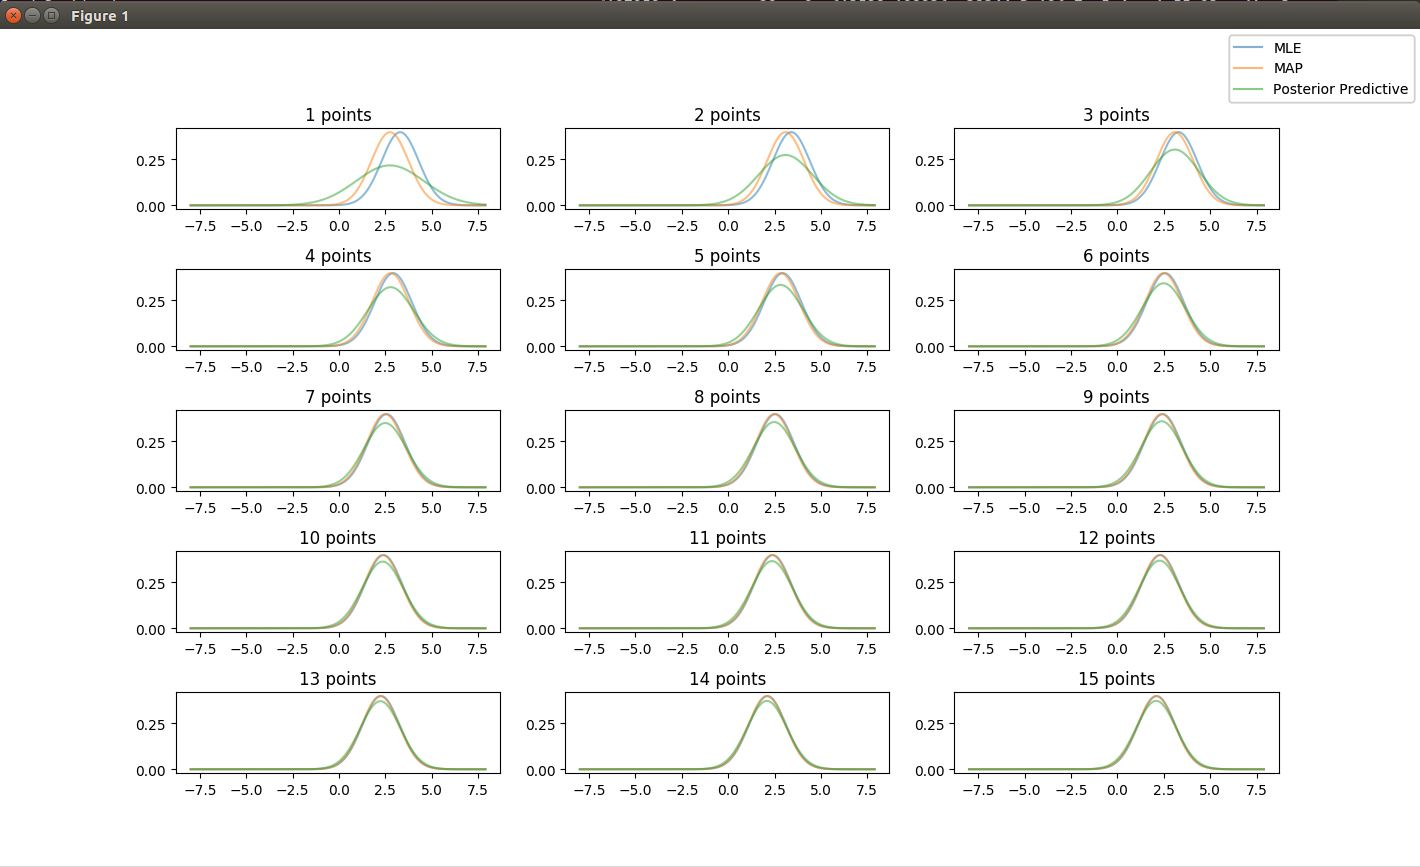
\includegraphics[scale=.50]{hw3/Pics/Capture.JPG}
     \item
     With more data the means of the predictive distributions converge to the actual mean of the data set. The variances of the MLE and MAP distributions do not change while the variance of the posterior predictive distribution narrows with more data.
     
     The MLE and MAP estimators have set variances that do not change which is why we see no change in the variance of the graphs. While the variance of the posterior predictive has a dependence on the data and number of data points which is why we see a significant narrowing.
     
     As for all the distributions we see that they converge to the mean by shifting left and right depending on the data points until all data points are included. We then get the result shown in the graphs.
     \item
     No the ordering does not matter because there is no dependence on order in any of the final predictive distributions.
     \item
     \begin{equation*}
         p(D) = \int p(D|\mu) p(\mu) d\mu
     \end{equation*}
     \begin{equation*}
        = \int \prod_{i} [\mcN(\mu, \sigma^2)] \mcN(0, \tau^2) d\mu
     \end{equation*}
     \begin{equation*}
        = \frac{1}{(\sqrt{2\pi}\sigma)^n(\sqrt{2\pi}\tau)}\int \exp(-\frac{1}{2\sigma^2}\sum_{i} (x_i - \mu)^2 - \frac{\mu^2}{2\tau^2}) d\mu
     \end{equation*}
     \begin{equation*}
        = \frac{1}{(\sqrt{2\pi}\sigma)^n(\sqrt{2\pi}\tau)}\int \exp(-\frac{1}{2\sigma^2}(\sum_{i} x_i^2 - 2\mu\sum_{i}x_i + \mu^2) - \frac{\mu^2}{2\tau^2}) d\mu
     \end{equation*}
     \begin{equation*}
        = \frac{\exp(-\frac{1}{2}(\frac{1}{\sigma^2}\sum_{i} x_i^2))}{(\sqrt{2\pi}\sigma)^n(\sqrt{2\pi}\tau)}\int \exp(-\frac{1}{2}(\frac{1}{\sigma^2}n\mu^2 - \frac{2}{\sigma^2}\sum_{i}x_i + \frac{\mu^2}{\tau^2})) d\mu
     \end{equation*}
     \begin{equation*}
        c = \frac{\exp(-\frac{1}{2}(\frac{1}{\sigma^2}\sum_{i} x_i^2))}{(\sqrt{2\pi}\sigma)^n(\sqrt{2\pi}\tau)}
     \end{equation*}
     \begin{equation*}
        = c\int \exp(-\frac{1}{2}(\frac{1}{\sigma^2}n\mu^2 - \frac{2}{\sigma^2}\sum_{i}x_i + \frac{\mu^2}{\tau^2})) d\mu
     \end{equation*}
     \begin{equation*}
        = c\int \exp(-\frac{1}{2}(\frac{n}{\sigma^2} + \frac{1}{\tau^2})(\mu^2 - 2\mu \frac{\frac{1}{\sigma^2}\sum_{i}x_i}{\frac{n}{\sigma^2} + \frac{1}{\tau^2}})) d\mu
     \end{equation*}
     \begin{equation*}
        = c \exp(\frac{(\frac{1}{\sigma^2}n\Bar{x})^2}{2(\frac{n}{\sigma^2} + \frac{1}{\tau^2})}) \int \exp(-\frac{1}{2}(\frac{n}{\sigma^2} + \frac{1}{\tau^2})(\mu - \frac{\frac{1}{\sigma^2}n\Bar{x}}{\frac{n}{\sigma^2} + \frac{1}{\tau^2}})^2) d\mu
     \end{equation*}
     \begin{equation*}
        = c \exp(\frac{(\frac{1}{\sigma^2}n\Bar{x})^2}{2(\frac{n}{\sigma^2} + \frac{1}{\tau^2})}) \frac{\sqrt{2\pi}}{\sqrt{\frac{n}{\sigma^2}+\frac{1}{\tau}}}
     \end{equation*}
     \begin{equation*}
        = \frac{\exp(-\frac{1}{2}(\frac{1}{\sigma^2}\sum_{i} x_i^2))}{(\sqrt{2\pi}\sigma)^n(\sqrt{2\pi}\tau)} \exp(\frac{(\frac{1}{\sigma^2}n\Bar{x})^2}{2(\frac{n}{\sigma^2} + \frac{1}{\tau^2})}) \frac{\sqrt{2\pi}}{\sqrt{\frac{n}{\sigma^2}+\frac{1}{\tau}}}
     \end{equation*}
     \begin{equation*}
        = \frac{\sigma}{(\sqrt{2\pi}\sigma)^n(\sqrt{n\tau^2 + \sigma^2})}\exp(-\frac{\sum_{i} x_i^2}{2\sigma^2})\exp(\frac{\tau^2 n^2\Bar{x}^2}{2\sigma^2(n\tau^2 + \sigma^2)})
     \end{equation*}
     \begin{center}
         Now substituting we get:
     \end{center}
     \begin{equation*}
        p(D) = \frac{\sigma}{(\sqrt{2\pi}\sigma)^n(\sqrt{n\tau^2 + \sigma^2})}\exp(-\frac{\sum_{i} x_i^2}{2\sigma^2})\exp(\frac{\tau^2 n^2\Bar{x}^2}{2\sigma^2(n\tau^2 + \sigma^2)}) = 4.4628725 \times 10^{-10}
     \end{equation*}
     \item \hspace{2cm}
     \begin{center}
         We can take our result from part 1.6 and just substitute in with $\tau = 0.1$
     \end{center}
     \begin{equation*}
        p(D) = \frac{\sigma}{(\sqrt{2\pi}\sigma)^n(\sqrt{n\tau^2 + \sigma^2})}\exp(-\frac{\sum_{i} x_i^2}{2\sigma^2})\exp(\frac{\tau^2 n^2\Bar{x}^2}{2\sigma^2(n\tau^2 + \sigma^2)}) = 7.9997049 \times 10^{-15}
     \end{equation*}
     
     The model where $\tau^2 = 5$ has a higher marginal likelihood.
     
     When we have a smaller $\tau^2$ we are more sure of the mean and as such the overall distribution of $\mu$ is much narrower and because of that our predictive distribution is integrated over a much smaller range of values and is smaller than when $\tau^2 = 5$.
 \end{enumerate}

\newpage
\begin{problem}[Backprop]

  In this problem, we will implement backprop for a simple MLP. The MLP will consist of a first fully connected layer with a sigmoid activation, followed by a one-dimensional, second fully connected layer with a sigmoid activation to get a prediction for a binary classification problem. Assume bias has not been merged. Let:
  \begin{itemize}
      \item $\bold{W}_1$ be the weights of the first layer, $\bold{b}_1$ be the bias of the first layer.
      \item $\bold{W}_2$ be the weights of the second layer, $\bold{b}_2$ be the bias of the second layer.
  \end{itemize}
  
  The described architecture can be written mathematically as: $$\hat{y} = \sigma(\bold{W}_2 \left[\sigma \left(\bold{W}_1 \bold{x} + \bold{b}_1\right)\right] + \bold{b}_2)$$
  
  where $\hat{y}$ is a scalar output of the net when passing in the single datapoint $\bold{x}$, the additions are element wise additions, and the sigmoid is an element wise sigmoid.
  
  \begin{enumerate}
      \item Let:
      \begin{itemize}
          \item $N$ be the number of datapoints we have
          \item $M$ be the dimensionality of the data
          \item $H$ be the size of the hidden dimension of the first layer. Here, hidden dimension is used to describe the dimension of the resulting value after going through the layer. Based on the problem description, the hidden dimension of the second layer should be 1.
      \end{itemize}
      
      Write out the dimensionality of each of the parameters, and of the intermediate variables:

          \begin{align*}
          \bold{a}_1 &= \bold{W}_1 \bold{x} + \bold{b}_1, 
          &\bold{z}_1 = \sigma(\bold{a}_1) \\
          a_2 &= \bold{W}_2 \bold{z}_1 + \bold{b}_2, 
          &\hat{y} = z_2 = \sigma(a_2)
          \end{align*}
          
      and make sure they work with the mathematical operations described above. Examining shapes is one of the key ways to debug your code, and can be done using .shape after any numpy array.
      
    \item  We will derive the gradient for each of the parameters before we implement backprop. For this question, assume there is only one datapoint $\bold{x}$, and that our loss is $L = y \log (\hat{y}) + (1 - y) \log (1 - \hat{y})$. For all questions, the chain rule will be useful.
    \begin{enumerate}
        \item Find $\frac{\partial L}{\partial b_2}$. 
        
        \item Find $\frac{\partial L}{\partial W_2^h}$, where $W_2^h$ represents the hth element of $\bold{W}_2$.
        
        \item Find $\frac{\partial L}{\partial b_1^h}$, where $b_1^h$ represents the hth element of $\bold{b}_1$. (*Hint: Note that only the hth element of $\bold{a}_1$ and $\bold{z}_1$ depend on $b_1^h$ - this should help you with how to use the chain rule.)
        
        \item Find $\frac{\partial L}{\partial W_1^{h,j}}$, where  $W_1^{h,j}$ represents the element in row $h$, column $j$ in $\bold{W}_1$.
    
    \end{enumerate}
    \end{enumerate}
    
    \end{problem}
    \setcounter{problem}{1}
    \begin{problem}[Backprop Cont.]
     Continued from previous page.
     
    \begin{enumerate}
     \setcounter{enumi}{2}
    
    \item Implement the gradient updates for the MLP with $H = 75$ with the given $\bold{X} \in \mathbb{R}^{N \times M}$ and $\bold{y} \in \mathbb{R}^N$ generated in the skeleton code for Q2 provided in the notebook. You will need to complete the forward and get$\_$grad functions. The get$\_$grad function should return the sum of each gradient over all (N) points. Feel free to use helper functions. Additionally, there is a PyTorch implementation of the gradient updates. PyTorch is Python library that supports automatic gradients (autograd), so the output of the torch implementation can be treated as a ground truth to compare to. Along with your code, include some screenshot showing your gradients match the torch autograd ones.
    
    If you are iterating through each datapoint and updating the parameters one element at a time (which is a good way to start!), note the time the updates takes. There are two places where we can vectorize our code to make it faster.
    \begin{enumerate}
        \item For each specific datapoint, we can update the entire gradient at once.  To get started on this, generalize your expression for $\frac{\partial L}{\partial W_2^h}$ to write an explicit expression for $\frac{\partial L}{\partial \bold{W}_2}$. Can you do similar things for the other gradient updates? 
        
        \item Then, we can batch gradient updates across all the datapoints.
    \end{enumerate}
    
    Update your code to be vectorized if it was not originally. For this question, the bulk of the speedup should come from the first vectorization and is the only part required. The second vectorization is bonus (and good practice!). How much speedup do you get (per one pass through the data)? If you don't have a baseline to compare to, the staff no vectorize solution took about 17s.
  
\end{enumerate}

\end{problem}
\newpage
\subsection*{Solution:}
\begin{enumerate}
    \item 
    $\boldx$: $M \times 1$\newline
    $\boldW_{1}$: $H \times M$\newline
    $\boldb_{1}$: $H \times 1$\newline
    $\bolda_{1}$: $H \times 1$\newline
    $\boldz_{1} = \sigma(\bolda_1)$: $H \times 1$\newline
    $\boldW_{2}$: $1 \times H$\newline
    $\boldb_{2}$: $1 \times 1$\newline
    $a_{2}$: $1 \times 1$\newline
    $\hat{y} = z_2 = \sigma(a_2)$: $1 \times 1$
    
    \item
    \begin{equation*}
        L = y \ln (\sigma(\bold{W}_2 \left[\sigma \left(\bold{W}_1 \bold{x} + \bold{b}_1\right)\right] + \bold{b}_2)) + (1 - y) \ln (1 - \sigma(\bold{W}_2 \left[\sigma \left(\bold{W}_1 \bold{x} + \bold{b}_1\right)\right] + \bold{b}_2))
    \end{equation*}
    \begin{enumerate}
        \item 
    \begin{equation*}
         \frac{\partial}{\partial b_2}(L = y \ln (\sigma(\bold{W}_2 \left[\sigma \left(\bold{W}_1 \bold{x} + \bold{b}_1\right)\right] + \bold{b}_2)) + (1 - y) \ln (1 - \sigma(\bold{W}_2 \left[\sigma \left(\bold{W}_1 \bold{x} + \bold{b}_1\right)\right] + \bold{b}_2)))
    \end{equation*}
    \begin{equation*}
         \frac{\partial L}{\partial b_2} = y (1 - \sigma(\bold{W}_2 \left[\sigma \left(\bold{W}_1 \bold{x} + \bold{b}_1\right)\right] + \bold{b}_2)) + (1 - y) \sigma(\bold{W}_2 \left[\sigma \left(\bold{W}_1 \bold{x} + \bold{b}_1\right)\right] + \bold{b}_2)
    \end{equation*}
    \item
    \begin{equation*}
        \frac{\partial}{\partial W_2^h}(L = y \ln (\sigma(\bold{W}_2 \left[\sigma \left(\bold{W}_1 \bold{x} + \bold{b}_1\right)\right] + \bold{b}_2)) + (1 - y) \ln (1 - \sigma(\bold{W}_2 \left[\sigma \left(\bold{W}_1 \bold{x} + \bold{b}_1\right)\right] + \bold{b}_2)))
    \end{equation*}
    \begin{equation*}
        \frac{\partial L}{\partial W_2^h} = y 
        (1 - \sigma(W_2^h \left[\sigma \left(\bold{W}_1^h \bold{x} + b_1^h\right)\right] + b_2^h)) (z_1^h) + (1 - y) (\sigma(W_2^h \left[\sigma \left(\bold{W}_1^h \bold{x} + b_1^h\right)\right] + b_2^h)(z_1^h)
    \end{equation*}
    \item
    \begin{equation*}    
        \frac{\partial}{\partial b_1^h}(L = y \ln (\sigma(\bold{W}_2 \left[\sigma \left(\bold{W}_1 \bold{x} + \bold{b}_1\right)\right] + \bold{b}_2)) + (1 - y) \ln (1 - \sigma(\bold{W}_2 \left[\sigma \left(\bold{W}_1 \bold{x} + \bold{b}_1\right)\right] + \bold{b}_2)))
    \end{equation*}
    \begin{equation*}
    \begin{split}
        \frac{\partial L}{\partial b_1^h} = y 
        (1-\sigma(W_2^h \left[\sigma \left(\bold{W}_1^h \bold{x} + b_1^h\right)\right] + b_2^h))
        W_2^h (\sigma(\bold{W}_1^h \bold{x} + b_1^h))(1-\sigma(\bold{W}_1^h \bold{x} + b_1^h)) \\ + (1 - y)(\sigma(W_2^h \left[\sigma \left(\bold{W}_1^h \bold{x} + b_1^h\right)\right] + b_2^h))
        W_2^h (\sigma(\bold{W}_1^h \bold{x} + b_1^h))(1-\sigma(\bold{W}_1^h \bold{x} + b_1^h))
       \end{split}
    \end{equation*}
    \item
    \begin{equation*}    
        \frac{\partial}{\partial W_1^{h,j}}(L = y \ln (\sigma(\bold{W}_2 \left[\sigma \left(\bold{W}_1 \bold{x} + \bold{b}_1\right)\right] + \bold{b}_2)) + (1 - y) \ln (1 - \sigma(\bold{W}_2 \left[\sigma \left(\bold{W}_1 \bold{x} + \bold{b}_1\right)\right] + \bold{b}_2)))
    \end{equation*}
    \begin{equation*}
        \begin{split}
        \frac{\partial L}{\partial W_1^{h,j}} = y 
        (1-\sigma(W_2^h \left[\sigma \left(W_1^{h,j} x^j + b_1^h\right)\right] + b_2^h))
        W_2^h (\sigma(W_1^{h,j} x^j + b_1^h))(1-\sigma(W_1^{h,j} x^j  + b_1^h)) \\ + (1 - y) (\sigma(W_2^h \left[\sigma \left(W_1^{h,j} x^j + b_1^h\right)\right] + b_2^h))
        W_2^h (\sigma(W_1^{h,j} x^j  + b_1^h))(1-\sigma(W_1^{h,j} x^j  + b_1^h))
        \end{split}
    \end{equation*}
    \end{enumerate}
    \newpage
    \item \hspace{2cm} \newline
    \begin{center}
       Truth \hspace{6cm} My Implementation
    \end{center}  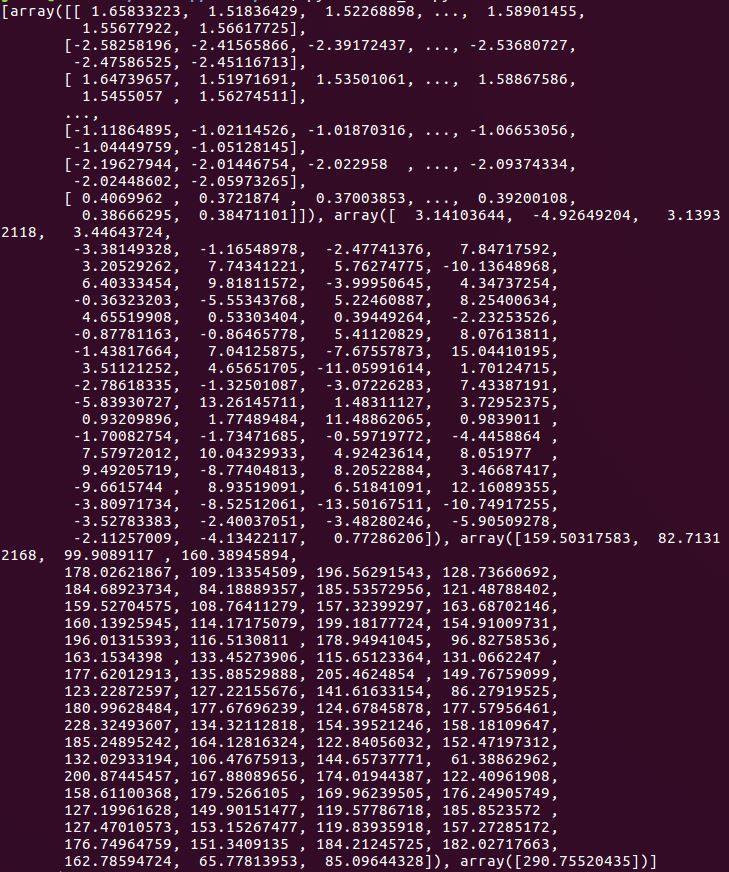
\includegraphics[scale=.50]{hw3/Pics/Capture3.JPG}
    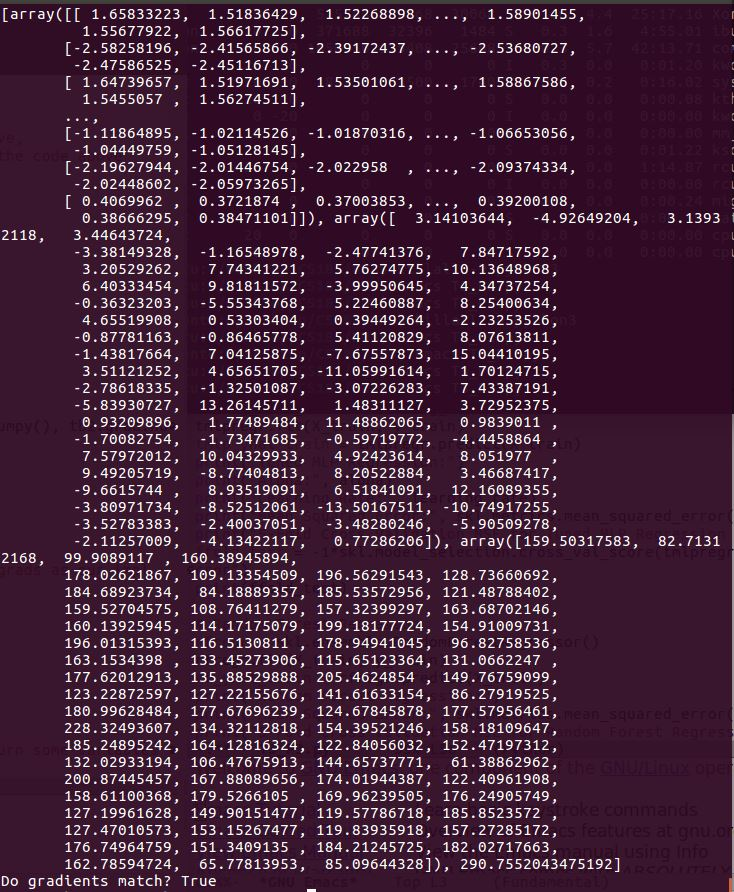
\includegraphics[scale=.50]{hw3/Pics/Capture2.JPG}
    The gradient calculation portion of my code takes 0.11170530319213867 seconds  to run. I did not do a non-vectorized solution so comparing to the staff solution time of about 17 seconds my gradient calculation is about 152 times faster.
\end{enumerate}


\newpage

\begin{problem}[Practical Supervised Learning]

  In this problem, we will try several methods on a real data set about housing prices in Boston. Each datapoint represents a town. There are 13 features including per-capita crime rate and teacher-student ratio. The target is the median value of a house in the town (in thousands). To measure performance, we will use MSE. We provide code to get the data and split the data into a train set and a test set in T3.py. Use the train split for all development (including validation and tuning). Use the test set to report final test performance (i.e. only for part 8).
  
  You may (and probably should) use existing software packages (e.g. sklearn) for this
  assignment.

\begin{enumerate}

  \item It's always good to start simple! Fit a linear regression to the train data and report train MSE. Then report a 5-fold cross validation MSE.
  
  \item Fit a ridge regression to the data and report train and cross-validation performance. Did this improve performance compared to linear regression? What does this tell you about our data and linear model?
  
  \item Examine the dataset. What sorts of data are there? Do you think a simple linear model models the data well? Hypothesize if more complex models that include non-linearities would improve performance.
    
  \item Fit a MLP Regressor to the dataset. Start with a 2-hidden-layer MLP with hidden sizes 75 each (i.e. pass in [75,75,] to the corresponding argument for the sklearn model). Report train and cross-validation performance. Compare the difference between train and validation performance for the MLP and for the previous linear models. Is this expected?
  
  \item Tune the MLP Regressor. One way you can tune is to do a grid search over certain hyperparameters. Report the relevant hyperparameters of your best model and the train and validation performance.

  \item Fit a Random Forest Regressor to the data and report train and validation performance. Both the Random Forest and MLP can capture non-linearities -- why do you think the difference in performance is what it is (some things to consider: dataset size, ease of training, tuning). 

  \item Tune for k and report the train and validation performance of your best kNN regressor. Why do you think kNN cannot match the performance of a MLP or Random Forest? How does kNN compare computationally to parametric methods during train time (especially as data set size increases)? What about during test time?
  
  \item Finally, report test performance for all the models mentioned previously. Comment briefly on validation vs. test performance.

\end{enumerate}

\end{problem}
\newpage

\subsection*{Solution:}
 \begin{enumerate}
     \item 
     Linear Regression Training Mean Squared Error: 19.272144590725716
     
    5-Fold Cross Validation MSE for Linear Regression Training Data: \newline 16.02794445, 48.50632367, 12.74195106, 11.69713358, 23.93173822
     \item
     Ridge Regression Training Mean Squared Error: 19.39246104909568

    5-Fold Cross Validation MSE for Ridge Regression Training Data: \newline 15.88977775, 49.21046253, 12.47407382, 11.79736241, 24.25631497
    
    No, ridge regression did not increase performance compared to linear regression. This tells us that our data is probably not well modeled by a linear model since adding regularization does not change the quality of the fit and predictions of our model.
    
    \item
    There are 13 variables overall. Some of those are numerical and some are categorical. Some of the numerical variables represent a linear relationship whereas some have no such relationship. A simple linear model would not perform well with this data. More complex models that could take into account more nuanced relationships between the variables would improve the performance.
    
    \item
    MLP Regression Training Mean Squared Error: 55.321936119912955
    
    5-Fold Cross Validation MSE for MLP Regression Training Data: \newline 33.21386913, 48.67184049, 32.38814759, 25.84562607, 33.29802893
    
    The MLP model gives both higher train and cross validation mean squared error. This is not expected because an MLP model should be able to account for non-linear relationships in our data. However this model is not tuned which is why we may be seeing the poorer performance relative to the linear models.
    
    \item\
    Hyperparameters:
    
    Alpha: 0.0001
    
    Learning Rate: 0.00001
    
    Solver: lbfgs
    
    Maximum iterations: 100000
    
    Activation function: relu
    
    Tuned MLP Regression Training Mean Squared Error: 2.4542575792572086
    
    5-Fold Cross Validation MSE for Tuned MLP Regression Training Data: \newline 11.02329679, 33.78367956,  9.08768975, 10.21991886, 29.85733865


    \item
    Random Forest Regression Training Mean Squared Error: 1.759140841584159

    5-Fold Cross Validation MSE for Random Forest Regression Training Data: \newline 7.33051056, 31.12830138,  6.58855442, 9.71850304, 17.97296579
    
    The Random Forest Regressor is a series of decision trees that can be trained fairly quickly when compared to MLP and captures the same if not more of the relationships than MLP. The Random Forest Regressor is also better at handling a smaller data set than that of the MLP Regressor. In addition, the MLP requires tuning to predict more correctly as shown in parts 4 and 5, and finding the hyperparameters that give the best fit is computationally expensive. That is not necessary with the Random Forest Regresssor which is another reason we see better overall performance from the Random Forest Regressor.
    
    \item
    Best Number of Neighbors: 2
    
    kNN Regression Training Mean Squared Error: 10.098601485148516
    
    5-Fold Cross Validation MSE for kNN Regression Training Data: \newline 38.16657407, 59.9512037,  31.35466049, 36.21453704, 31.79921875
    
    kNN uses the neighbors to predict the value of the variable, but with a data set so complex and with so many features the nearest neighbors may not be very representative of the actual value.
    
    kNN is computationally faster than parametric models at train time because it performs a series of comparisons and averages. Whereas parametric model must calculate computationally expensive equations in order to train the model, this becomes especially apparent once the data becomes very large. 
    
    During test time they all perform about the same speed because the model has already been trained and the steps needed to calculate a prediction are relatively computationally non-intensive.
    
    \item
    Linear Regression Test Data:
    
    Mean Squared Error: 38.782960960846694
    
    Ridge Regression Test Data:
    
    Mean Squared Error: 39.66375959063913
    
    MLP Regression Test Data:
    
    Mean Squared Error: 97.4941502907401
    
    Tuned MLP Regression Test Data:
    
    Mean Squared Error: 17.765996390510573
    
    Random Forest Regression Test Data:
    
    Mean Squared Error: 15.572669196078419
    
    kNN Regression Test Data:
    
    Mean Squared Error: 58.06419117647059

    We see the linear models perform worse with the novel test data because they are not great at predicting the non-linear relationships present in the data. We also see the kNN model performs worse relative to the training performance because the nearest neighbors are not necessarily the best predictors of the actual value of the novel data. The untrained MLP Regressor obviously performs poorly in both cases since it is untrained. Lastly, we see that the two parametric models, the Tuned MLP Regressor and the Random Forest Regressor, both perform the best, in training and testing, since they can best model the relationships in the training data and generalize to the novel test data.
 \end{enumerate}
\newpage
%%%%%%%%%%%%%%%%%%%%%%%%%%%%%%%%%%%%%%%%%%%%%
% Name and Calibration
%%%%%%%%%%%%%%%%%%%%%%%%%%%%%%%%%%%%%%%%%%%%%
\subsection*{Name}

Jason Sibrian

\subsection*{Collaborators and Resources}
Whom did you work with, and did you use any resources beyond cs181-textbook and your notes?

https://www.cs.ubc.ca/~murphyk/Papers/bayesGauss.pdf for help on Posterior Predictive

\subsection*{Calibration}
Approximately how long did this homework take you to complete (in hours)? 

45


\end{document}

